\documentclass[final,12pt]{elsarticle}

\usepackage{amsmath}
\usepackage{amssymb}
\usepackage{booktabs}
\usepackage{enumitem}
\usepackage{float}
\usepackage{graphicx}
\usepackage{microtype}
\usepackage{multirow}
\usepackage[section]{placeins}
\usepackage{xcolor}
\usepackage[hidelinks]{hyperref}
\usepackage[nameinlink,noabbrev]{cleveref}
\emergencystretch=2em

% Supplementary numbering: Table S1..., Figure S1...
\renewcommand{\thetable}{S\arabic{table}}
\renewcommand{\thefigure}{S\arabic{figure}}

\newcommand{\systemname}{ConstructionSceneReady}

\journal{Automation in Construction}

\begin{document}

\begin{frontmatter}
\title{Supplementary Material:\\ConstructionSceneReady: Evidence-grounded
compilation and task-scene validation for BIM-driven robotic assembly}
\begin{abstract}
This supplementary file collects the larger mapping, registry, design,
ablation, and per-condition statistics tables, plus the worked case-study
figure, referenced from the main manuscript. Table and figure numbers carry
an ``S'' prefix and are cited from the main text as Table~S1\ldots S8 and
Figure~S9.
\end{abstract}
\end{frontmatter}

\section{Supplementary tables}
\label{app:tables}

This appendix collects the larger mapping, registry, design, and
ablation tables referenced from the main text.

\begin{table*}[!tbp]
\centering
\caption{Task-information mapping for the bolt-insertion assembly task. For
each building-information family: the robot function it serves, the task
phase in which it acts, and the measured consequence of its absence or error
(\Cref{sec:task-outcomes}). ``Scaffolded'' marks families whose dynamical
channel is removed by the virtual-grasp executor; their task consequence is
explicitly \emph{not} claimed by this study.}
\label{tab:info-mapping}
\small
\resizebox{\textwidth}{!}{%
\begin{tabular}{p{0.16\textwidth}p{0.24\textwidth}p{0.14\textwidth}p{0.36\textwidth}}
\toprule
Information family & Robot function served & Task phase & Measured consequence
of defect \\
\midrule
Semantic identity \& task reference & Select which member, interface and hole
to act on & target selection & \emph{wrong} value discretely fatal (0\%);
\emph{missing} label degrades (12.0\% reward, 1.0\% geo.); no perceptual
compensation for a wrong target \\
Member pose (absolute) & Coarse approach and reach planning & transport &
largely compensated: reward $-$4.5\,pp (significant on seed 42,
$p{=}0.012$), geo.\ $-$2.0\,pp (n.s.) \\
Interface coordinates relative to member & Fine alignment at the hole mouth
& align, insert & reward-tolerance partly masks it ($-$1.0\,pp at 2--5\,mm,
n.s.) but geometric-valid degrades strongly ($-$12.5/$-$14.0\,pp at 2/5\,mm,
$-41.5$\,pp at 10\,mm) \\
Interface clearance \& tolerance & Physical insertability of the fastener
& insert & sensitive continuous feature; $-$54.5\,pp reward at 0.75\,mm
clearance \\
Construction state \& sequence & Gate whether the action is legal now &
precondition check & discretely fatal (0\%) \\
Physical properties (mass, friction) & Force-level contact and stability &
contact stages & \emph{scaffolded}: no dynamical channel in the
transport-and-insert executor (bit-identical outcomes); not ranked \\
\bottomrule
\end{tabular}
}
\end{table*}

\begin{table*}[!tbp]
\centering
\caption{Provenance of task information: source class, extraction, runtime
use, and repair responsibility. IFC-native = present in the delivery;
derived = computed from IFC geometry/material; task annotation = CSR
property-set/robot--task specification; assumed = default that must be
escalated, never silently trusted.}
\label{tab:info-provenance}
\small
\resizebox{\textwidth}{!}{%
\begin{tabular}{p{0.20\textwidth}p{0.14\textwidth}p{0.24\textwidth}p{0.20\textwidth}p{0.14\textwidth}}
\toprule
Field & Source class & Extraction & Runtime use & Repair source \\
\midrule
Component identity / IFC GUID & IFC-native & preserved through compilation &
cross-reference closure & IFC source \\
Member pose (absolute) & IFC-native & \texttt{IfcLocalPlacement} $\rightarrow$
USD transform & transport target pose & IFC source \\
Interface coordinates (hole, member-relative) & derived & IFC hole feature
$\rightarrow$ evidence record & fine alignment at hole mouth & evidence
record \\
Interface clearance / tolerance & task annotation & CSR property set $\rightarrow$
evidence record + provenance & geometric insertability gate & evidence
record \\
Construction state / sequence & task annotation & task state machine &
precondition gate & task file \\
Mass / inertia & derived & IFC volume $\times$ material density (+uncertainty)
& physics stability & derived value \\
Work zone / payload & task annotation & CSR property set & multi-scale
activation & task file \\
Robot capability / preconditions & task annotation & robot--task specification
& executor configuration & task file \\
Unannotated required field & \emph{assumed} & none (absent) & none $\rightarrow$
escalate & human review \\
\bottomrule
\end{tabular}
}
\end{table*}

\begin{table*}[!tbp]
\centering
\caption{Construction-scene readiness contract (v0.3.0). The frozen v0.2.0
set carries 30 rules (CSR-SCN-001--030); v0.3.0 adds CSR-SCN-031 and
CSR-SCN-032 for evidence-grounded interface fidelity, 32 rules in total. The
versioned registry is exported at \texttt{docs/scene-readiness-rules.csv},
and per-scenario coverage is reported in the supplementary material.}
\label{tab:contract}
\small
\resizebox{\textwidth}{!}{%
\begin{tabular}{p{0.16\textwidth}p{0.23\textwidth}p{0.19\textwidth}
p{0.10\textwidth}p{0.22\textwidth}}
\toprule
Contract category & Required scene evidence & Deterministic check &
Severity & Consequence if violated \\
\midrule
Identity and closure & IFC GUID, USD prim path, closed task and asset
references & Uniqueness and reference resolution & Critical & Wrong or
unresolved task object \\
Spatial consistency & Units, up axis, frames, transform chain, work-zone
membership & Transform normalization and bounds & Critical & Unreachable or
misplaced interaction \\
Assembly interface & Paired interface, insertion axis, tolerance, grasp and
support regions & Geometric and relational constraints & Critical & False
alignment or infeasible insertion \\
Construction state & Current state, legal predecessor, action precondition,
completion criterion & State-machine validation & Critical & Unsafe or
meaningless action \\
Physics and stability & Mass, inertia, collision, contact property, temporary
support & Physical admissibility and support tests & Critical or major & Unstable
or non-physical simulation \\
Provenance and fidelity & Property source, confidence, uncertainty, activated
payload and level of detail & Authority and task-fidelity policy & Major &
Unauditable result or hidden interaction error \\
\bottomrule
\end{tabular}
}
\end{table*}

\begin{table*}[!tbp]
\centering
\caption{Benchmark composition. Faulted-case counts are read from the frozen
partition manifest (\texttt{data/partition-manifest.json}): 9 development, 24
test, and 2 challenge faults per scenario scene, with test and challenge
faults evaluated on held-out geometric variants. All scenarios are exercised
end-to-end at the compile--validate--repair level; robot execution in this
paper is reported for the pin-insertion scenario at the fixed-base level,
and the remaining scenario$\,\times\,$level combinations are the benchmark's
intended progression.}
\label{tab:benchmark}
\small
\resizebox{\textwidth}{!}{%
\begin{tabular}{p{0.19\textwidth}p{0.22\textwidth}p{0.18\textwidth}
p{0.14\textwidth}p{0.17\textwidth}}
\toprule
Scenario & Parameterization & Robot task levels & Faulted cases &
Primary outcome \\
\midrule
Connection-plate positioning & Component size, pose, target height,
work-zone obstacle & Fixed base; whole body; mobile & 9 dev / 24 test / 2 challenge & Placement pose and state completion \\
Simplified pin insertion & Interface axis, clearance, friction, initial
misalignment & Fixed base (executed here); whole body, mobile (progression) & 9 dev / 24 test / 2 challenge & Insertion depth without jam \\
Sequential assembly & Component order, temporary support, path obstruction,
state transition & Fixed base; whole body; mobile & 9 dev / 24 test / 2 challenge & Complete legal task sequence \\
\bottomrule
\end{tabular}
}
\end{table*}

\begin{table*}[!tbp]
\centering
\caption{Ablation and sensitivity analysis relative to the fixed-rule row of
\Cref{tab:detection-repair} (105 paired cases each; bootstrap 95\% CIs in
brackets). The first four columns are measured on the ablated pipeline
 itself. The last column is \emph{not} an ablation effect: it is the index of
the \emph{related} defect-consequence condition from \Cref{sec:task-outcomes}
that conceptually matches the removed information, shown only to indicate how
consequential that information family is at runtime (removing provenance is
not the same as corrupting a physical value, and removing the task validator
is not the same as every scene having a wrong task reference).}
\label{tab:ablation}
\small
\resizebox{\textwidth}{!}{%
\begin{tabular}{p{0.24\textwidth}p{0.23\textwidth}cccc}
\toprule
Ablation & Removed information or control & Critical recall & Valid repair &
Resource use & Related defect outcome \\
\midrule
No provenance & Source authority and uncertainty & 0.894 [0.839, 0.941] &
85.7\% [79.0, 92.4] & unchanged & 87.0\% (physics, non-consequential) \\
No task validator & Task binding and action preconditions &
0.787 [0.706, 0.868] & 80.0\% [72.4, 87.6] & unchanged & 0.0\% (task
reference, fatal) \\
All layers loaded & Task-triggered payload activation & 1.000 & 97.1\% &
+27\% prims, +20\% layer bytes & n/a \\
Fixed repair order & Agentic tool selection & 1.000 & 97.1\% & unchanged &
identical to fixed rule \\
Free-form diagnostics & Typed diagnostic schema & 1.000 (given) &
89.0\% [86.3, 91.6] & unchanged & n/a \\
\bottomrule
\end{tabular}
}
\end{table*}

\begin{table*}[t]
\centering
\caption{Repair outcome by frozen partition (development 27 / test 72 /
challenge 6 cases; agent rows 5 seeds per case). Development cases are
repaired to pristine equivalence by both grounded methods and test cases
nearly all (fixed-rule 100.0\%, constrained agent 99.4\%); the challenge
cases---whose repair would exceed the available engineering evidence---are
split three repaired and three escalated by design, and never incorrectly
repaired. The unconstrained agent fails across all partitions with a
substantial incorrect-repair share.}
\label{tab:partition-repair}
\small
\begin{tabular}{p{0.24\textwidth}cccc}
\toprule
Method & Dev valid (27) & Test valid (72) & Challenge valid (6) &
Challenge escalated \\
\midrule
Fixed-rule conversion & 100.0\% & 100.0\% & 50.0\% & 50.0\% \\
Validator-grounded agent & 100.0\% & 99.4\% & 50.0\% & 50.0\% \\
Unconstrained agent & 40.0\% & 32.8\% & 0.0\% & 80.0\% \\
\bottomrule
\end{tabular}
\\[2pt]
{\footnotesize Incorrect repair is 0.0\% in every partition for the
fixed-rule and validator-grounded rows; the unconstrained agent's incorrect
share is 19.3\%/24.2\%/20.0\% (dev/test/challenge).}
\end{table*}

\begin{table*}[t]
\centering
\caption{Runtime resource use and task-level outcomes. Resource cells are
reported per composition mode on the held-out variant scenes (structural
metrics are exact; load time is the median of five cold opens and varies with
host). Peak memory stayed below the 1\,MB measurement threshold. Task stages
are measured with the frozen RL executor on the defect-free scene (the cell
reports the seed-42 partition; the seed-123 value is 84.0\%,
\Cref{tab:geo-condition-stats}); planning, grasp, and alignment are not
instrumented
separately under the virtual-grasp scaffold (\Cref{sec:task-outcomes}).}
\label{tab:runtime-task}
\small
\resizebox{\textwidth}{!}{%
\begin{tabular}{p{0.17\textwidth}cccccccc}
\toprule
Condition & Active prims & Peak memory & Load time & Planning & Grasp &
Alignment & Insertion & Full task \\
\midrule
Direct/all loaded & 28--30 & $<$1\,MB & 1.4\,ms & n/a & n/a & n/a & n/a &
n/a \\
Fixed rule & \multicolumn{4}{l}{identical compiler output as full method} &
n/a & n/a & n/a & n/a \\
Free-form agent & \multicolumn{8}{l}{method-independent compilation output;
task cells not instrumented (\Cref{sec:task-outcomes})} \\
Full/task activated & 22--24 & $<$1\,MB & 1.5\,ms & n/a & n/a & n/a &
87.0\% (seed 42) & = insertion \\
\bottomrule
\end{tabular}
}
\end{table*}



\begin{table}[H]
\centering
\caption{Per-condition geometric-valid statistics behind
\Cref{tab:readiness-confusion}: 200 paired episodes per condition and seed
partition, defect-free versus defect scene geometric-valid successes
(ok${\rightarrow}$def), discordant pairs $b$/$c$ (lost/gained), and exact
two-sided McNemar $p$; (a) seed 42, (b) seed 123. \emph{Validator} names the
rule that fires on the condition's contract-equivalent fault (v0.2.0;
mapping in the text); \emph{silent} conditions violate no declared rule.
Cells: TP\,=\,flagged and consequential; FN\,=\,silent but consequential;
TN\,=\,silent, no significant degradation detected in the batch;
FP\,=\,flagged without detected degradation (none occurred). Generated from
the per-episode ledgers of \Cref{tab:defect-decay}.}
\label{tab:geo-condition-stats}
\scriptsize
\setlength{\tabcolsep}{2.5pt}
\textbf{(a) seed 42}\\[2pt]
\begin{tabular}{ll ccl c}
\toprule
Condition & rule & ok${\rightarrow}$def & $b$/$c$ & $p$ & cell \\
\midrule
hole $+$2\,mm & silent & 87$\rightarrow$62 & 44/19 & 0.0022 & FN \\
hole $+$5\,mm & silent & 87$\rightarrow$59 & 53/25 & 0.0020 & FN \\
hole $+$10\,mm & silent & 87$\rightarrow$4 & 85/2 & 4.9e-23 & FN \\
member $+$10\,mm & silent & 87$\rightarrow$83 & 29/25 & 0.68 & TN \\
clear.\ 0.75\,mm & silent & 87$\rightarrow$65 & 41/19 & 0.0062 & FN \\
clear.\ 0.5\,mm & silent & 87$\rightarrow$41 & 52/6 & 3.2e-10 & FN \\
clear.\ 0.25\,mm & silent & 87$\rightarrow$15 & 74/2 & 7.7e-20 & FN \\
sem.\ missing & SCN-003 & 87$\rightarrow$2 & 85/0 & 5.2e-26 & TP \\
sem.\ wrong & SCN-004 & 87$\rightarrow$0 & 87/0 & 1.3e-26 & TP \\
task ref. & SCN-028 & 87$\rightarrow$0 & 87/0 & 1.3e-26 & TP \\
state & SCN-021 & 87$\rightarrow$0 & 87/0 & 1.3e-26 & TP \\
mass $\times0.5$ & silent & 87$\rightarrow$87 & 0/0 & 1.0 & TN \\
mass $\times2$ & silent & 87$\rightarrow$87 & 0/0 & 1.0 & TN \\
\bottomrule
\end{tabular}\\[6pt]
\textbf{(b) seed 123}\\[2pt]
\begin{tabular}{ll ccl c}
\toprule
Condition & rule & ok${\rightarrow}$def & $b$/$c$ & $p$ & cell \\
\midrule
hole $+$2\,mm & silent & 86$\rightarrow$77 & 39/30 & 0.34 & TN \\
hole $+$5\,mm & silent & 86$\rightarrow$62 & 53/29 & 0.011 & FN \\
hole $+$10\,mm & silent & 86$\rightarrow$11 & 82/7 & 2.4e-17 & FN \\
member $+$10\,mm & silent & 86$\rightarrow$74 & 41/29 & 0.19 & TN \\
clear.\ 0.75\,mm & silent & 86$\rightarrow$57 & 42/13 & 1.1e-4 & FN \\
clear.\ 0.5\,mm & silent & 86$\rightarrow$36 & 58/8 & 1.8e-10 & FN \\
clear.\ 0.25\,mm & silent & 86$\rightarrow$11 & 76/1 & 1.0e-21 & FN \\
sem.\ missing & SCN-003 & 86$\rightarrow$0 & 86/0 & 2.6e-26 & TP \\
sem.\ wrong & SCN-004 & 86$\rightarrow$0 & 86/0 & 2.6e-26 & TP \\
task ref. & SCN-028 & 86$\rightarrow$0 & 86/0 & 2.6e-26 & TP \\
state & SCN-021 & 86$\rightarrow$0 & 86/0 & 2.6e-26 & TP \\
mass $\times0.5$ & silent & 86$\rightarrow$86 & 0/0 & 1.0 & TN \\
mass $\times2$ & silent & 86$\rightarrow$86 & 0/0 & 1.0 & TN \\
\bottomrule
\end{tabular}
\end{table}


\begin{figure*}[t]
\centering
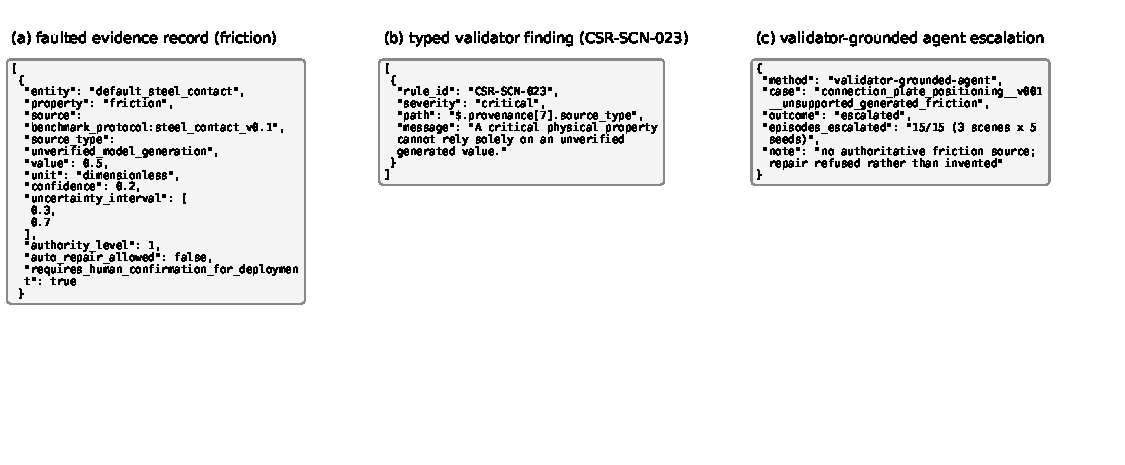
\includegraphics[width=\textwidth]{figures/fig09_case_study.pdf}
\caption{Auditable failure--diagnosis--escalation sequence for the held-out
challenge case \texttt{unsupported\_generated\_friction}
(\texttt{connection\_plate\_positioning\_\_v001}). (a) The faulted provenance record: friction
entered by unverified model generation with low confidence and repair blocked
by policy. (b) The deterministic typed finding (CSR-SCN-023). (c) The frozen
validator-grounded model escalates in all 15 episodes rather than inventing a
friction value. All panels render committed artefacts (scene JSON, validation
report, episode ledger) via \texttt{scripts/make\_case\_study\_figure.py}.}
\label{fig:case-study}
\end{figure*}


\end{document}
